% \documentclass[]{tMOP2e}
% 
% \citestyle{tMOP}
% \begin{document}
% 
% \doi{10.1080/0950034YYxxxxxxxx}
% \issn{1362-3044}
% \issnp{0950-0340} \jvol{00} \jnum{00} \jyear{2010} \jmonth{25 January}

%\markboth{A. Yamilov and B. Payne}{Lorem ipsum dolor sit amet, consectetur adipiscing elit. Maecenas ultrices egestas commodo.}
 
\chapter{Classification of regimes of wave transport in quasi one-dimensional non-conservative random media}
\label{chap:regimes}
\label{paper:2_start}

% \author{
% A. Yamilov$^\ast$ \thanks{$^\ast$Corresponding author. Email: yamilov@mst.edu \vspace{6pt}} and 
% B. Payne\\\vspace{6pt}  {\em{Physics Department, Missouri University of Science and Technology, Rolla, MO USA}}}
% 
\begin{center}
Alexey Yamilov$^1$ and Ben Payne$^1$
\end{center}

\ \\
\begin{center}
\textit{$^1$Department of Physics, Missouri University of Science \& Technology,\\ Rolla, MO 65409}
%$^2$Department of Applied Physics, Yale University, New Haven, CT 06520}
\end{center}

\ \\
% \maketitle
% \begin{abstract}
% 
\addcontentsline{toc}{section}{ABSTRACT}
\begin{center}\textbf{ABSTRACT\footnote{Published in Journal of Modern Optics (2010)}}        \end{center}

Passive quasi-one-dimensional random media are known to exhibit one of the three regimes of transport -- ballistic, diffusive or localized --  depending on the system size. In contrast, in non-conservative systems the physical parameter space also includes the gain/absorption length scale. Here, by studying the relationships between the transport mean free path, the localization length, and the gain/absorption length, we enumerate fifteen regimes of wave propagation through quasi-one-dimensional random media with gain or absorption. The results are presented graphically in a form of a phase diagram. Of particular experimental importance, in absorbing random medium we identify three different regimes which bear signatures of the localized regime of the passive counterpart. We also review the literature and, when possible, assign experimental systems to a particular regime on the diagram. 
% \begin{keywords} 
% Wave propagation in random media; diffusion; Anderson localization; random laser
% \end{keywords}
% \end{abstract}

\section{INTRODUCTION}
\label{sec:introduction}

Discovery of Anderson localization (AL)~\cite{1958_Anderson}Lorem ipsum dolor sit amet, consectetur adipiscing elit. Maecenas ultrices egestas commodo.~\cite{2009_Lagendijk_PT}. AL is a wave phenomenon~\cite{2007_Akkermans_book} that results in cessation of diffusion~\cite{2010_Wolfle}. First conceived in electronic systems,Lorem ipsum dolor sit amet, consectetur adipiscing elit. Maecenas ultrices egestas commodo. Conservation of number of carriers,Lorem ipsum dolor sit amet, consectetur adipiscing elit. Maecenas ultrices egestas commodo, lies in the foundation of the concept of AL~\cite{1991_Altshuler}. 

Understanding the effect of absorption~\cite{1984_John_prl}, ubiquitous in optical systems,Lorem ipsum dolor sit amet, consectetur adipiscing elit. Maecenas ultrices egestas commodo.{\it light}~\cite{1989_Genack,1997_wiersma_nature,1999_Maret,2000_chabanov_nature,2007_Maret,2007_Segev} and other classical waves such as ultrasound~\cite{2008_van_Tiggelen_Nature,2008_Weaver}. It also prompted~\cite{2000_chabanov_nature}Lorem ipsum dolor sit amet, consectetur adipiscing elit. Maecenas ultrices egestas commodo. Furthermore, the effect opposite to the absorption, coherent amplification,Lorem ipsum dolor sit amet, consectetur adipiscing elit. Maecenas ultrices egestas commodo.~\cite{2005_Cao,2008_Wiersma}. Lorem ipsum dolor sit amet, consectetur adipiscing elit. Maecenas ultrices egestas commodo,Lorem ipsum dolor sit amet, consectetur adipiscing elit. Maecenas ultrices egestas commodo,Lorem ipsum dolor sit amet, consectetur adipiscing elit. Maecenas ultrices egestas commodo. Lorem ipsum dolor sit amet, consectetur adipiscing elit. Maecenas ultrices egestas commodo.~\cite{2010_Payne_loc_criterion}.

In this work,Lorem ipsum dolor sit amet, consectetur adipiscing elit. Maecenas ultrices egestas commodo.(quasi-1D) random media, such as disordered waveguides,Lorem ipsum dolor sit amet, consectetur adipiscing elit. Maecenas ultrices egestas commodo. In quasi-1D geometry the transition to AL lacks sharp features (mobility edges) observed in even more complex three-dimensional systems. Thus,  Section \ref{sec:q1d_localization}Lorem ipsum dolor sit amet, consectetur adipiscing elit. Maecenas ultrices egestas commodo.1D random media. In Section \ref{sec:parameters}Lorem ipsum dolor sit amet, consectetur adipiscing elit. Maecenas ultrices egestas commodo.1D non-conservative systems. In Section \ref{sec:phases},Lorem ipsum dolor sit amet, consectetur adipiscing elit. Maecenas ultrices egestas commodo. Furthermore, we review the available publications on the subject and, when published data is sufficient, assign them to a particular region on our phase-diagram. Lorem ipsum dolor sit amet, consectetur adipiscing elit. Maecenas ultrices egestas commodo.\ref{sec:discussion}.

\section{LOCALIZATION IN QUASI-1D NON-CONSERVATIVE RANDOM MEDIA}
\label{sec:q1d_localization}

\subsection{Localization in Finite Passive Random Media}

Lorem ipsum dolor sit amet, consectetur adipiscing elit. Maecenas ultrices egestas commodo.~\cite{2010_Spencer}. In experimentally relevant situations,Lorem ipsum dolor sit amet, consectetur adipiscing elit. Maecenas ultrices egestas commodo. Thus,Lorem ipsum dolor sit amet, consectetur adipiscing elit. Maecenas ultrices egestas commodo. 

Lorem ipsum dolor sit amet, consectetur adipiscing elit. Maecenas ultrices egestas commodo, but microscopically different disorder realizations, $g$,Lorem ipsum dolor sit amet, consectetur adipiscing elit. Maecenas ultrices egestas commodo.~\cite{1977_Thouless}. According to scaling theory of localization~\cite{1979_Anderson}, $g$Lorem ipsum dolor sit amet, consectetur adipiscing elit. Maecenas ultrices egestas commodo, formally described by the scaling function~\cite{2010_Kramer}. Thus,Lorem ipsum dolor sit amet, consectetur adipiscing elit. Maecenas ultrices egestas commodo.

are listed in Table~\ref{tab:c}. Out of six possible couplings only three appear to be important including one next-nearest coupling. The latter corresponds to coupling between the diagonal cavities in the diamond arrangement.

\begin{table}
\begin{center}
\caption{\label{tab:c}Coupling coefficients for nearest and next-nearest pairings}
\begin{tabular}{||c|c|c||c|c|c||}
\hline
$c^{(nn)}_{1}$ & $c^{(nn)}_{2}$ & $c^{(nn)}_{3}$ & $c^{(nnn)}_{1}$ & $c^{(nnn)}_{2}$ & $c^{(nnn)}_{3}$ \\ \hline
$0.004105$ & $0.000915$ & $0.000238$ & $0.002034$ & $0.000736$ & $0.000261$ \\
% from /svn/research/Project_DAS/2012_TB_for_2DTM_manuscript/TB_for_2DTM.xlsx SVN 3082
\hline
\end{tabular}
\end{center}
\end{table}

\subsection{Localization in Finite Random Media With Gain or Absorption}

Lorem ipsum dolor sit amet, consectetur adipiscing elit. Maecenas ultrices egestas commodo.~\cite{1988_Stone}. Lorem ipsum dolor sit amet, consectetur adipiscing elit. Maecenas ultrices egestas commodo.(LC) based on $g$ in optical systems. However,Lorem ipsum dolor sit amet, consectetur adipiscing elit. Maecenas ultrices egestas commodo,Lorem ipsum dolor sit amet, consectetur adipiscing elit. Maecenas ultrices egestas commodo.~\cite{1999_van_Tiggelen}. Lorem ipsum dolor sit amet, consectetur adipiscing elit. Maecenas ultrices egestas commodo.~\cite{1994_Freilikher_absorption}. Indeed, in absorbing systems $g\ll 1$ may not be indicative of the presence of localization~\cite{1998_Brouwer,2000_chabanov_nature}, and $g\gg 1$Lorem ipsum dolor sit amet, consectetur adipiscing elit. Maecenas ultrices egestas commodo.~\cite{2004_Yamilov_intensity,2006_Yamilov_conductance}. Therefore,Lorem ipsum dolor sit amet, consectetur adipiscing elit. Maecenas ultrices egestas commodo.~\cite{1994_Kumar,1995_Zhang,1996_Paasschens_gain,1997_Freilikher_gain,1998_Maret_PRL,2000_chabanov_nature,2006_Yamilov_conductance}, rounding of the coherent back scattering cone~\cite{1997_Wiersma_cbs,1999_Kaiser_cbs,2009_Maret}, anomalous diffusion~\cite{1989_Genack,1997_wiersma_nature,2006_Maret,2007_Segev,2008_van_Tiggelen_Nature,2009_Genack_PRB} and others.

In the case of absorption, a quantitative criterion, based on the magnitude of {\it fluctuation} of transmission normalized by its average, was put forward~\cite{2000_chabanov_nature}. Although it described the experiment well,Lorem ipsum dolor sit amet, consectetur adipiscing elit. Maecenas ultrices egestas commodo. Lorem ipsum dolor sit amet, consectetur adipiscing elit. Maecenas ultrices egestas commodo.~\cite{1994_Freilikher_absorption},Lorem ipsum dolor sit amet, consectetur adipiscing elit. Maecenas ultrices egestas commodo. 

In random media with gain,Lorem ipsum dolor sit amet, consectetur adipiscing elit. Maecenas ultrices egestas commodo. Without saturation effects,Lorem ipsum dolor sit amet, consectetur adipiscing elit. Maecenas ultrices egestas commodo. Lorem ipsum dolor sit amet, consectetur adipiscing elit. Maecenas ultrices egestas commodo. To regularize the statistical ensemble,Lorem ipsum dolor sit amet, consectetur adipiscing elit. Maecenas ultrices egestas commodo.~\cite{2005_Yamilov_correlations}. Lorem ipsum dolor sit amet, consectetur adipiscing elit. Maecenas ultrices egestas commodo.~\cite{2004_Yamilov_intensity,2006_Yamilov_conductance,2005_Yamilov_correlations}. It was found that the correlation linewidth $\delta\omega$~\cite{2000_Sebbah}Lorem ipsum dolor sit amet, consectetur adipiscing elit. Maecenas ultrices egestas commodo.$\delta=\delta\omega/\Delta\omega$ in random media with gain. Here $\Delta\omega$Lorem ipsum dolor sit amet, consectetur adipiscing elit. Maecenas ultrices egestas commodo.  Reduction of $\delta$ correlates well~\cite{2005_Yamilov_correlations}Lorem ipsum dolor sit amet, consectetur adipiscing elit. Maecenas ultrices egestas commodo. Lorem ipsum dolor sit amet, consectetur adipiscing elit. Maecenas ultrices egestas commodo. Lorem ipsum dolor sit amet, consectetur adipiscing elit. Maecenas ultrices egestas commodo, the relationship $g=\delta$ is no longer valid in non-conservative media. Lorem ipsum dolor sit amet, consectetur adipiscing elit. Maecenas ultrices egestas commodo(or absorption),Lorem ipsum dolor sit amet, consectetur adipiscing elit. Maecenas ultrices egestas commodo(see e.g. Refs.~\cite{1999_Patra_noise,2009_Skipetrov_noise}) are not accounted for.

\subsection{Disordered Waveguide (Wire) Geometry}

Lorem ipsum dolor sit amet, consectetur adipiscing elit. Maecenas ultrices egestas commodo, the transport properties in quasi-1D (waveguide) Lorem ipsum dolor sit amet, consectetur adipiscing elit. Maecenas ultrices egestas commodo~\cite{1997_Beenakker}. Lorem ipsum dolor sit amet, consectetur adipiscing elit. Maecenas ultrices egestas commodo~\cite{2004_Mello_Kumar_book} which yielded some exact analytical results~\cite{1994_Beenakker_exact,2000_Mirlin}.

In passive quasi-1Lorem ipsum dolor sit amet, consectetur adipiscing elit. Maecenas ultrices egestas commodo$L$ only (and not the strength of disorder as in three-dimensions, 3D), even if the system is weakly scattering $k\ell\gg 1$. The diffusion regime is only a transitive regime which, unlike in 3D systems, does not persists in the limit $L\rightarrow\infty$. Therefore, quasi-1D systems 
\cite{1995_Kogan,1996_Paasschens_gain,1998_Brouwer,1998_Birman_waveguide,1998_Maret_PRL,1999_Muttalib,
2000_chabanov_nature,2002_Saenz_g,2005_Markos,2005_Genack_review,2006_Yamilov_conductance,2007_Botten_waveguide,
2007_Froufe-Perez_PRE,2007_deMatos_random_fiber_laser}Lorem ipsum dolor sit amet, consectetur adipiscing elit. Maecenas ultrices egestas commodo. However,Lorem ipsum dolor sit amet, consectetur adipiscing elit. Maecenas ultrices egestas commodo$L\rightarrow\infty$ may not be easily defined, quasi-1Lorem ipsum dolor sit amet, consectetur adipiscing elit. Maecenas ultrices egestas commodo{\it finite size}. As shown below, it is expected to exhibit very complex parameter space, c.f. Fig.~\ref{fig:phase_space}. Furthermore,Lorem ipsum dolor sit amet, consectetur adipiscing elit. Maecenas ultrices egestas commodo,Lorem ipsum dolor sit amet, consectetur adipiscing elit. Maecenas ultrices egestas commodo1D non-conservative random media. 

Lorem ipsum dolor sit amet, consectetur adipiscing elit. Maecenas ultrices egestas commodo(see e.g. Refs.~\cite{1994_Kumar,1995_Zhang,1995_zyuzin_fluctuations,1996_Paasschens_gain,1997_Freilikher_gain,1997_Wiersma_cbs,
2000_Cao_localization,2001_Soukoulis_modeDist,2001_Sebbah_FDTD,2004_Yamilov_intensity,2005_Genack_Milner,
2005_Apalkov_corr,2005_Yamilov_correlations,2006_Heinrichs,2006_Yamilov_conductance,2008_Stone,2008_Conti_opals,
2009_Frank,2010_Payne_PRL}),Lorem ipsum dolor sit amet, consectetur adipiscing elit. Maecenas ultrices egestas commodo. Below,Lorem ipsum dolor sit amet, consectetur adipiscing elit. Maecenas ultrices egestas commodo1D non-conservative random media.

%-----------------------------------------------
\section{DEFINITIONS OF PARAMETERS IN QUASI-1D NON- CONSERVATIVE RANDOM MEDIA}
\label{sec:parameters}
%-----------------------------------------------

%%%%%%%%%%%%%%%%%%%%%%%%%%%%%%%%%%%%%%%%%%%%
\begin{figure}
\vskip -0.2cm
\centerline{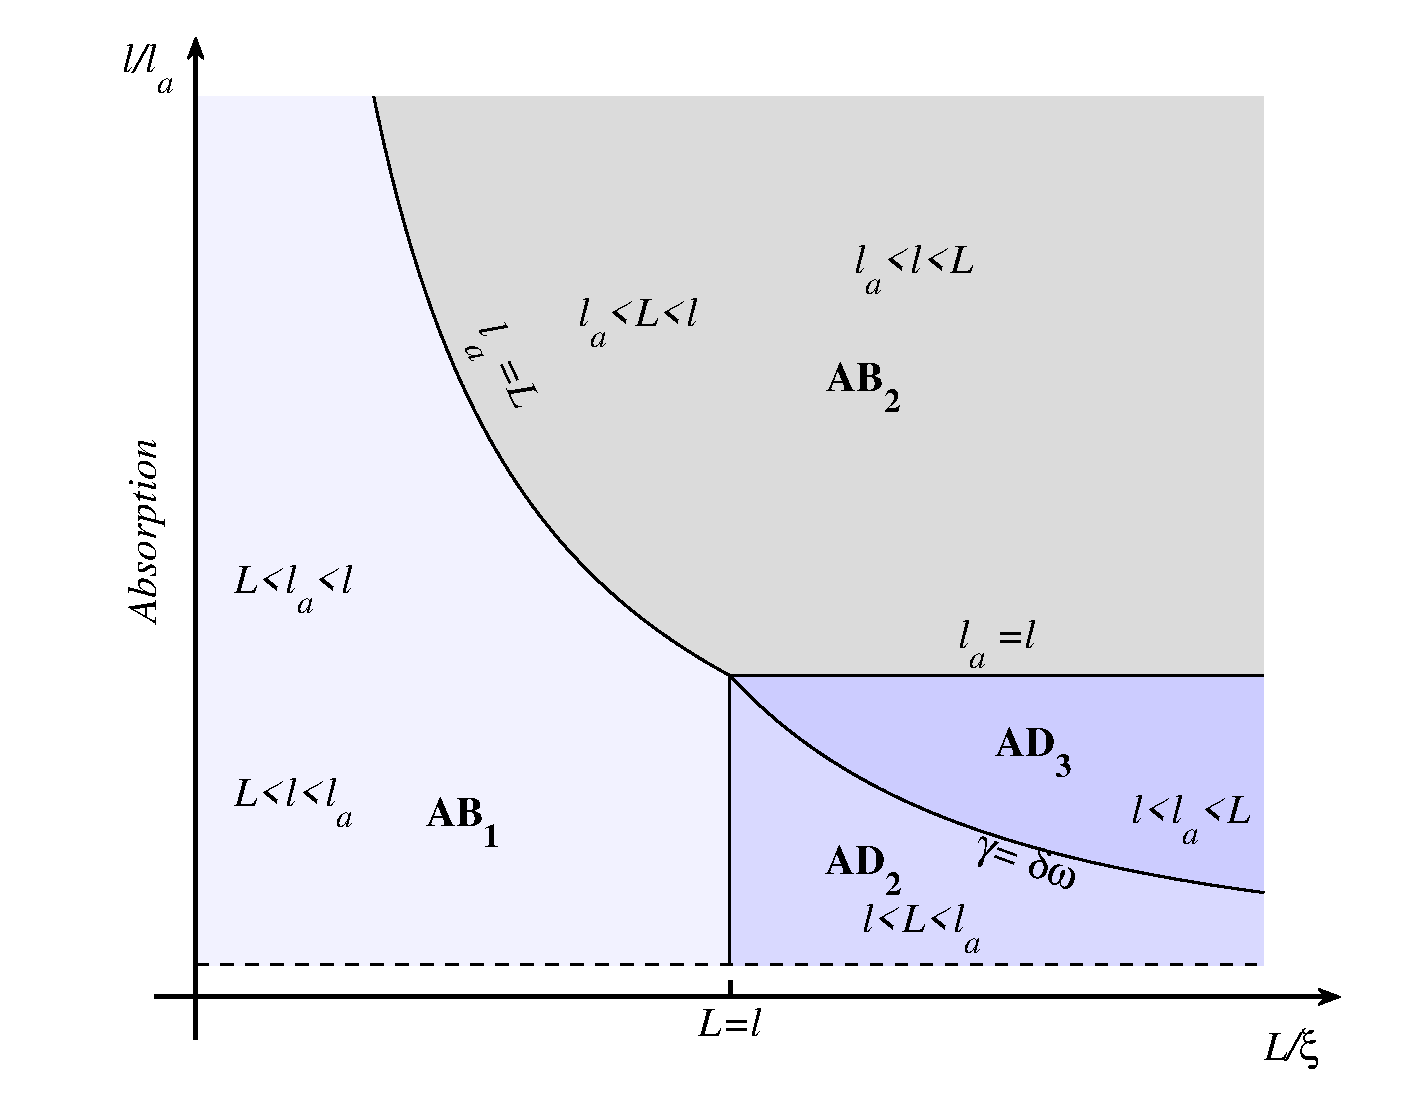
\includegraphics[width=4in]{chapters/paper2_fdsa/pictures/fig1a_regimes_plot_upper}}
\vskip -0.2cm
\caption[Classification of regimes of wave transport in quasi-1D non-conservative random media; upper panel.]{Classification of regimes of wave transport in quasi-1D non-conservative random media; upper panel.}
\end{figure}

\begin{figure}
\hskip -0.1cm
\centerline{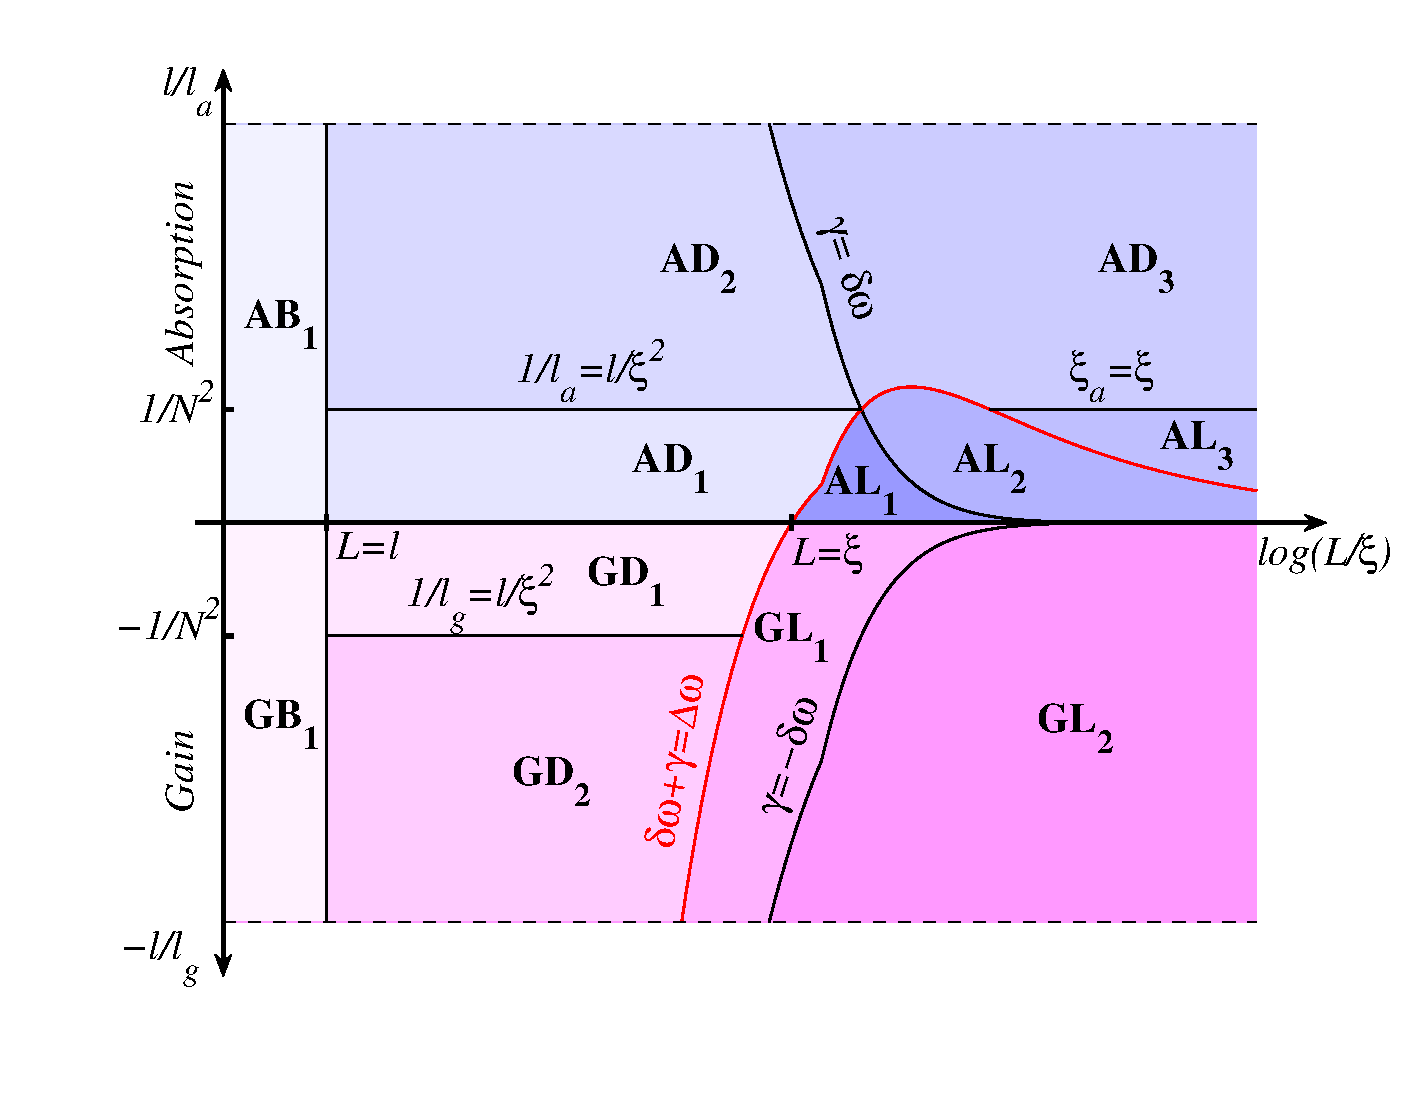
\includegraphics[width=4.15in]{chapters/paper2_fdsa/pictures/fig1b_regimes_plot_main}}
\caption[Classification of regimes of wave transport in quasi-1D non-conservative random media; middle panel.]{Classification of regimes of wave transport in quasi-1D non-conservative random media; middle panel.}
\end{figure}

\begin{figure}
\vskip -0.6cm
\centerline{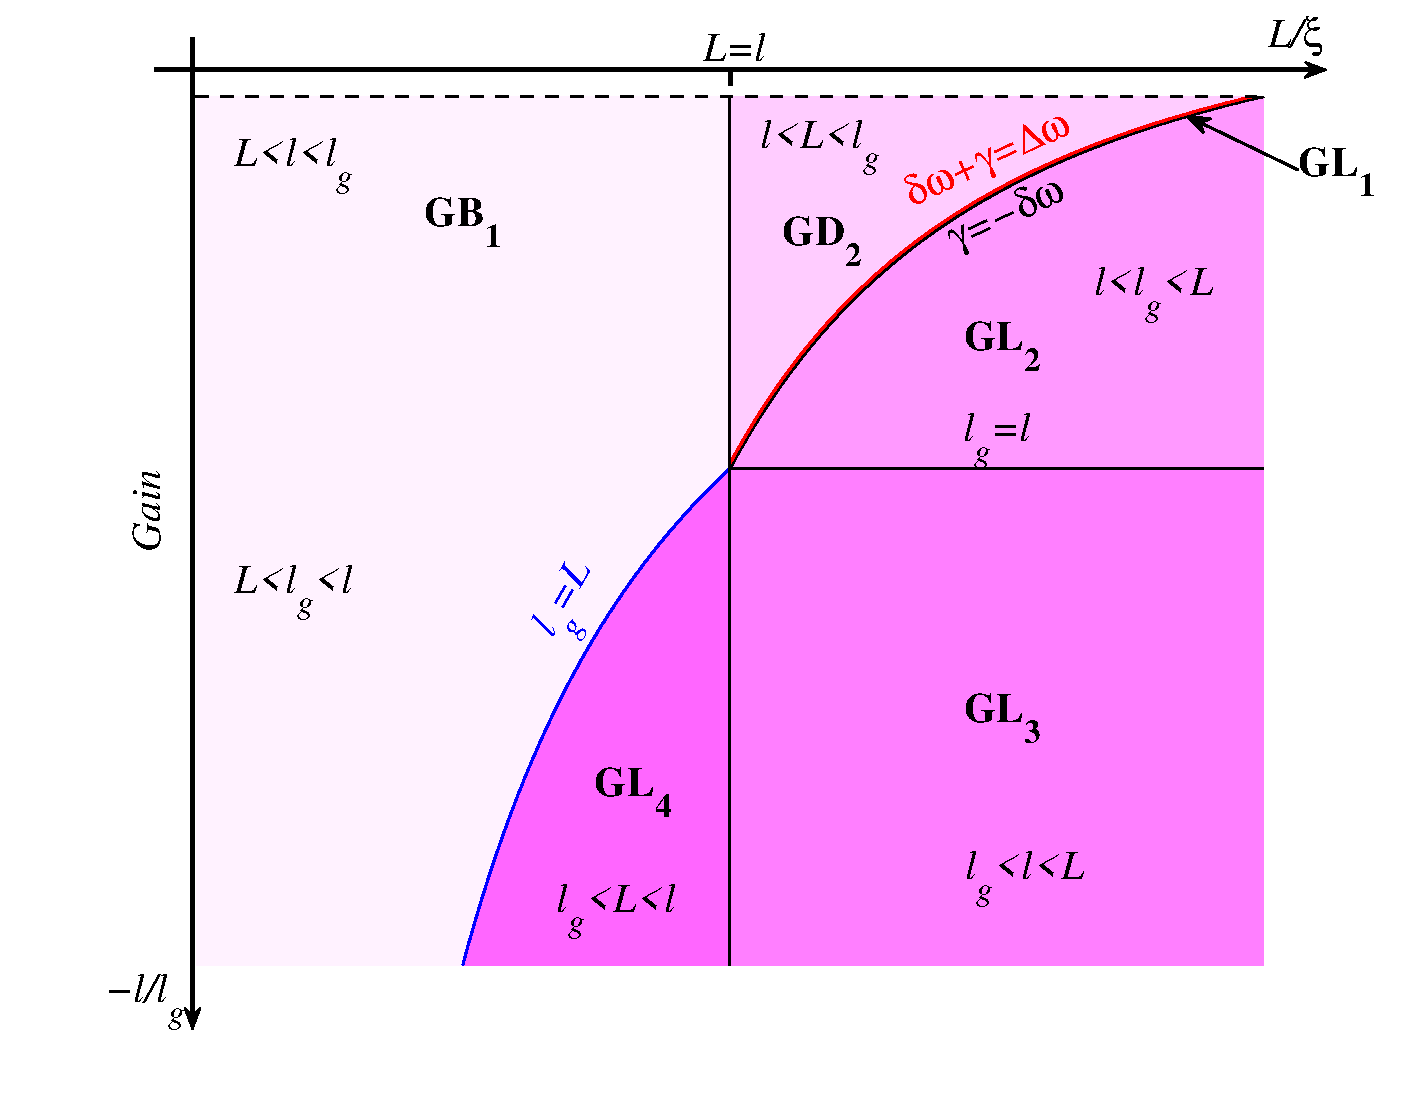
\includegraphics[width=4in]{chapters/paper2_fdsa/pictures/fig1c_regimes_plot_lower}}
\vskip -0.2cm
\caption[Classification of regimes of wave transport in quasi-1D non-conservative random media; lower panel.]{\label{fig:phase_space} Classification of regimes of wave transport in quasi-1D non-conservative random media; lower panel. X and Y axes correspond to the system length $L$ and absorption/gain length $\ell_{a,g}$, see text for labeling convention. Due to large disparity in the characteristic length scales, the plot is separated into three panels which correspond to strong absorption $1/\ell_a\sim 1/\ell$ (upper panel), weak absorption and gain $1/\ell_{a,g}\sim \ell/\xi^2$ (middle panel), and strong gain $1/\ell_g\sim 1/\ell$ (lower panel) regimes. }
\end{figure}
%%%%%%%%%%%%%%%%%%%%%%%%%%%%%%%%%%%%%%%%%%%%%

In passive volume-disordered waveguides,Lorem ipsum dolor sit amet, consectetur adipiscing elit. Maecenas ultrices egestas commodo$\ell$ and $\xi=N\times\ell$ respectively. Here $\ell$ is the transport mean free path, $N$ is the number of waveguide channels, and $\xi$ is the localization length~\cite{1997_Beenakker}. In waveguides filled with a non-conservative random medium, the parameter space becomes two-dimensional: beside the system size $L$, it also includes the gain or absorption length scale $\ell_{g,a}$. Fig.~\ref{fig:phase_space} shows this two-parameter phase space.

The boundaries between different regions in Fig.~\ref{fig:phase_space}Lorem ipsum dolor sit amet, consectetur adipiscing elit. Maecenas ultrices egestas commodo. The length parameters include $L$, $\ell$, $\xi$, and (ballistic) absorption/gain lengths $\ell_a/\ell_g$. Lorem ipsum dolor sit amet, consectetur adipiscing elit. Maecenas ultrices egestas commodo: the average mode spacing $\Delta\omega\propto (NL)^{-1}$; the passive average mode linewidth $\delta\omega$ ($\propto DL^{-2}$ in diffusive regime $\ell<L<\xi$); and gain or absorption rate $\gamma_{g,a}=\mp c/\ell_{g,a}\equiv\mp\tau_{g,a}^{-1}$ (negative in the case of gain). Here, $c$ is speed of light and $D$ is the diffusion constant. Lorem ipsum dolor sit amet, consectetur adipiscing elit. Maecenas ultrices egestas commodo:
\begin{quote}
$\bullet$ $L\sim\ell$Lorem ipsum dolor sit amet, consectetur adipiscing elit. Maecenas ultrices egestas commodo. Lorem ipsum dolor sit amet, consectetur adipiscing elit. Maecenas ultrices egestas commodo/gain $\ell<\ell_{g,a}$ shown in the middle panel in Fig.~\ref{fig:phase_space};\\
$\bullet$ Generalized Thouless parameter $\delta\omega(\gamma)/\Delta\omega\simeq(\delta\omega+\gamma)/\Delta\omega$ describes~\cite{2005_Yamilov_correlations}Lorem ipsum dolor sit amet, consectetur adipiscing elit. Maecenas ultrices egestas commodo. Here $\delta\omega\equiv\delta\omega(\gamma=0)$. In the case of passive system $\gamma=0$, the ratio reduces to $\delta=g$;\\
$\bullet$ $|\gamma|=\delta\omega$Lorem ipsum dolor sit amet, consectetur adipiscing elit. Maecenas ultrices egestas commodo;\\
$\bullet$Lorem ipsum dolor sit amet, consectetur adipiscing elit. Maecenas ultrices egestas commodo. In quasi-1D, the probability of such paths becomes equal to unity at $L=\xi$, their length is given by $L^2/\ell=\xi^2/\ell$. Therefore,Lorem ipsum dolor sit amet, consectetur adipiscing elit. Maecenas ultrices egestas commodo$\ell_{g,a}$ becomes comparable to this length scale;\\
$\bullet$ Condition $\ell=\ell_{g,a}$ marks the onset of the regimes of very strong absorption/gain shown in the upper/lower panel in Fig.~\ref{fig:phase_space}. Here, the ballistic regimes become limited by the condition $\ell_{g,a}=L$.\\
\end{quote}
Lorem ipsum dolor sit amet, consectetur adipiscing elit. Maecenas ultrices egestas commodo. When gain is present, the statistical ensemble is assumed to be conditional~\cite{2005_Yamilov_correlations}, which excludes the non-physical solutions~\cite{2002_Zhang_phys_solutions}. Furthermore, the considered (open) system is of a finite size and, therefore, the transitions between different ``phases'' are expected to be smooth. Hence,Lorem ipsum dolor sit amet, consectetur adipiscing elit. Maecenas ultrices egestas commodo.

\section{``PHASES'' OF WAVE TRANSPORT THROUGH \\NON-CONSERVATIVE RANDOM MEDIA} 
\label{sec:phases}

The regions in Fig.~\ref{fig:phase_space} are labeled with two letters and a subscript. The first letter, $A/G$, stand for {\underline a}bsorption/{\underline g}ain and is common for all regions above/below the horizontal axis. The second letter in the labels, $B$, $D$ or $L$, is attributed to the regimes where some signatures of the {\underline b}allistic, {\underline d}iffusive, and {\underline l}ocalized transport are expected to occur. Based on the list of separatrices listed above, one can identify the following regions:
\begin{quote}
$\bullet$ $GB_1,AB_1$:Lorem ipsum dolor sit amet, consectetur adipiscing elit. Maecenas ultrices egestas commodo. Note that in the regime of very strong gain or absorption, $\ell_{g,a}^{-1}>\ell^{-1}$, the ballistic region becomes bounded by $L<\ell_{g,a}$;\\
$\bullet$ $GD_1,AD_1$: With exception of anomalously localized states~\cite{1991_Altshuler,1995_Muzykantskii_ALS,2000_Mirlin,2000_Cao_localization,2002_Apalkov_ALS,2004_Burin_ALS},Lorem ipsum dolor sit amet, consectetur adipiscing elit. Maecenas ultrices egestas commodo; \\
$\bullet$ $GD_2$: Such systems were successfully treated with the ``negative absorption''Lorem ipsum dolor sit amet, consectetur adipiscing elit. Maecenas ultrices egestas commodo~\cite{1968_Letokhov,1994_lawandy_nature,1996_John_RandLaser,1996_Wiersma_RandomLaser,1996_Genack_DiffRandomLaser,
1999_Cao_RandomLaserPRL,1999_Vardeny_PolymerRandomLaser,2001_vansoest_thesis,2004_Florescu}. Lorem ipsum dolor sit amet, consectetur adipiscing elit. Maecenas ultrices egestas commodo~\cite{2005_Yamilov_correlations,2004_Yamilov_intensity,2006_Yamilov_conductance};\\
$\bullet$ $GL_1$: Random media with such strong gain, $\delta\omega(\gamma)/\Delta\omega<1$,Lorem ipsum dolor sit amet, consectetur adipiscing elit. Maecenas ultrices egestas commodo~\cite{1995_zyuzin_fluctuations,1997_Burkov_Zyuzin}. Lorem ipsum dolor sit amet, consectetur adipiscing elit. Maecenas ultrices egestas commodo~\cite{1999_Jiang,2002_Zhang_phys_solutions} for the systems with the parameters in this region;\\
$\bullet$ $GL_2$: The condition $\gamma_g=-\delta\omega(\gamma =0)$ signifies lasing of an average mode and, in diffusive systems,Lorem ipsum dolor sit amet, consectetur adipiscing elit. Maecenas ultrices egestas commodo~\cite{1968_Letokhov}; \\
$\bullet$ $AL_1,AL_2,AL_3$:Lorem ipsum dolor sit amet, consectetur adipiscing elit. Maecenas ultrices egestas commodo. Of these, $AL_1$Lorem ipsum dolor sit amet, consectetur adipiscing elit. Maecenas ultrices egestas commodo, $\delta\omega(\gamma)/\Delta\omega\simeq(\delta\omega(\gamma=0)+\gamma)/\Delta\omega<1$,Lorem ipsum dolor sit amet, consectetur adipiscing elit. Maecenas ultrices egestas commodo(possibly, experimental systems of~\cite{2000_chabanov_nature} belong to this parameter ``phase''). The latter is no longer true for $AL_2$ regime. $AL_3$Lorem ipsum dolor sit amet, consectetur adipiscing elit. Maecenas ultrices egestas commodo, but still exhibiting the weak localization corrections;\\
$\bullet$ $AD_2,AD_3$:Lorem ipsum dolor sit amet, consectetur adipiscing elit. Maecenas ultrices egestas commodo~\cite{1998_Brouwer}. For strong absorption,Lorem ipsum dolor sit amet, consectetur adipiscing elit. Maecenas ultrices egestas commodo. Lorem ipsum dolor sit amet, consectetur adipiscing elit. Maecenas ultrices egestas commodo;\\
$\bullet$ $AB_2$:Lorem ipsum dolor sit amet, consectetur adipiscing elit. Maecenas ultrices egestas commodo$\ell_a$ is the shortest of all length-scales. Because it also implies $\ell_a^{-1}>\ell^{-1}$, diffusion-like propagation does not sets in;\\
$\bullet$ $GL_3,GL_4$: In these regimes, similar to $GL_2$, it is more meaningful to ascribe $L$ notation to {\underline l}asing. In contrast to the very strong absorption counterpart $AB_2$, we separated $\ell_g^{-1}>\ell^{-1}$ region into $\ell_g<\ell<L$ ($GL_3$) and $\ell_g<L<\ell$ ($GL_4$). In the latter regime, one can justify neglecting scattering. Thus, $GL_4$ encompasses lasing phenomena in Fabry-Perot geometry. In contrast, in $GL_3$Lorem ipsum dolor sit amet, consectetur adipiscing elit. Maecenas ultrices egestas commodo~\cite{2006_Wu,2006_Wu_spie}.\\
\end{quote}
% Unlike the absorbing systems where one loc-abs, gain diff-loc\\

\section{DISCUSSION AND OUTLOOK}
\label{sec:discussion_regimes}

As it was discussed in the previous section,Lorem ipsum dolor sit amet, consectetur adipiscing elit. Maecenas ultrices egestas commodo. Importantly, the coherent amplification/Lorem ipsum dolor sit amet, consectetur adipiscing elit. Maecenas ultrices egestas commodo, thus, can promote/suppress localization phenomena. Lorem ipsum dolor sit amet, consectetur adipiscing elit. Maecenas ultrices egestas commodo~\cite{1995_zyuzin_fluctuations,1997_Burkov_Zyuzin,2004_Yamilov_intensity,2005_Yamilov_correlations,2006_Yamilov_conductance,2010_Payne_loc_criterion,2010_Payne_TE}. Furthermore, in the experimental studies of localization of light,Lorem ipsum dolor sit amet, consectetur adipiscing elit. Maecenas ultrices egestas commodo~\cite{1991_Genack,1997_wiersma_nature,1999_Maret,2000_chabanov_nature,2006_Maret}. 

In finite {\it passive} random media,Lorem ipsum dolor sit amet, consectetur adipiscing elit. Maecenas ultrices egestas commodo: averaged dimensional conductance, its mesoscopic fluctuations relative to the mean value, Thouless parameter, renormalization of the diffusion coefficient, inverse participation ratio, spatial correlations and others. Lorem ipsum dolor sit amet, consectetur adipiscing elit. Maecenas ultrices egestas commodo. Lorem ipsum dolor sit amet, consectetur adipiscing elit. Maecenas ultrices egestas commodo. We believe that our analysis of the parameter space in Sec.~\ref{sec:phases}Lorem ipsum dolor sit amet, consectetur adipiscing elit. Maecenas ultrices egestas commodo{\it non-conservative} random media~\cite{2010_Payne_loc_criterion,2010_Payne_TE}.

\section{ACKNOWLEDGMENTS}
Lorem ipsum dolor sit amet, consectetur adipiscing elit. Maecenas ultrices egestas commodo. DMR-0704981. 
%Lorem ipsum dolor sit amet, consectetur adipiscing elit. Maecenas ultrices egestas commodo, award no. DMR-090132.

